\documentclass[
  bibliography=totoc,     % Literatur im Inhaltsverzeichnis
  captions=tableheading,  % Tabellenüberschriften
  titlepage=firstiscover, % Titelseite ist Deckblatt
]{scrartcl}
% Paket float verbessern
\usepackage{scrhack}

% Warnung, falls nochmal kompiliert werden muss
\usepackage[aux]{rerunfilecheck}

% unverzichtbare Mathe-Befehle
\usepackage{amsmath}
% viele Mathe-Symbole
\usepackage{amssymb}
% Erweiterungen für amsmath
\usepackage{mathtools}

% Fonteinstellungen
\usepackage{fontspec}
% Latin Modern Fonts werden automatisch geladen
% Alternativ zum Beispiel:
%\setromanfont{Libertinus Serif}
%\setsansfont{Libertinus Sans}
%\setmonofont{Libertinus Mono}

% Wenn man andere Schriftarten gesetzt hat,
% sollte man das Seiten-Layout neu berechnen lassen
\recalctypearea{}

% deutsche Spracheinstellungen
\usepackage[ngerman]{babel}


\usepackage[
  math-style=ISO,    % ┐
  bold-style=ISO,    % │
  sans-style=italic, % │ ISO-Standard folgen
  nabla=upright,     % │
  partial=upright,   % ┘
  warnings-off={           % ┐
    mathtools-colon,       % │ unnötige Warnungen ausschalten
    mathtools-overbracket, % │
  },                       % ┘
]{unicode-math}

% traditionelle Fonts für Mathematik
\setmathfont{Latin Modern Math}
% Alternativ zum Beispiel:
%\setmathfont{Libertinus Math}

\setmathfont{XITS Math}[range={scr, bfscr}]
\setmathfont{XITS Math}[range={cal, bfcal}, StylisticSet=1]

% Zahlen und Einheiten
\usepackage[
  locale=DE,                   % deutsche Einstellungen
  separate-uncertainty=true,   % immer Unsicherheit mit \pm
  per-mode=symbol-or-fraction, % / in inline math, fraction in display math
]{siunitx}

% chemische Formeln
\usepackage[
  version=4,
  math-greek=default, % ┐ mit unicode-math zusammenarbeiten
  text-greek=default, % ┘
]{mhchem}

% richtige Anführungszeichen
\usepackage[autostyle]{csquotes}

% schöne Brüche im Text
\usepackage{xfrac}

% Standardplatzierung für Floats einstellen
\usepackage{float}
\floatplacement{figure}{htbp}
\floatplacement{table}{htbp}

% Floats innerhalb einer Section halten
\usepackage[
  section, % Floats innerhalb der Section halten
  below,   % unterhalb der Section aber auf der selben Seite ist ok
]{placeins}

% Seite drehen für breite Tabellen: landscape Umgebung
\usepackage{pdflscape}

% Captions schöner machen.
\usepackage[
  labelfont=bf,        % Tabelle x: Abbildung y: ist jetzt fett
  font=small,          % Schrift etwas kleiner als Dokument
  width=0.9\textwidth, % maximale Breite einer Caption schmaler
]{caption}
% subfigure, subtable, subref
\usepackage{subcaption}

% Grafiken können eingebunden werden
\usepackage{graphicx}

% schöne Tabellen
\usepackage{booktabs}

% Verbesserungen am Schriftbild
\usepackage{microtype}

% Literaturverzeichnis
\usepackage[
  backend=biber,
]{biblatex}


% Hyperlinks im Dokument
\usepackage[
  german,
  unicode,        % Unicode in PDF-Attributen erlauben
  pdfusetitle,    % Titel, Autoren und Datum als PDF-Attribute
  pdfcreator={},  % ┐ PDF-Attribute säubern
  pdfproducer={}, % ┘
]{hyperref}
% erweiterte Bookmarks im PDF
\usepackage{bookmark}

% Trennung von Wörtern mit Strichen
\usepackage[shortcuts]{extdash}

%Tabelle aus .txt
%\usepackage{pgfplotstable}

\author{%
  Frederik Zielke\\%
  \href{mailto:frederik.zielke@tu-dortmund.de}{frederik.zielke@tu-dortmund.de}%
  \and%
  Lennart Völz\\%
  \href{mailto:lennart.voelz@tu-dortmund.de}{lennart.voelz@tu-dortmund.de}%
}
\publishers{TU Dortmund – Fakultät Physik}

% Quellendatenbank
\addbibresource{lit.bib}
\addbibresource{programme.bib}

\subject{V354}
\title{Gedämpfte und erzwungene Schwingungen}
\date{%
  Durchführung: 10.01.23
  \hspace{3em}
  Abgabe: 17.01.23
}

\begin{document}
\setlength{\parindent}{0pt} %kein Einrücken mehr

\maketitle
\thispagestyle{empty}
\tableofcontents
\newpage

\section{Theorie}
\label{sec:Theorie}

\subsection{Kräfte}
Auf Körper die sich durch eine Flüssigkeit bewegen wirkt eine Reibungskraft $\vec{F}$,
die der Bewegungsrichtung entegengesetzt ist. Die Reibungskraft ist Abhängig von der Berührungsfläche A,
der Geschwindigkeit $v$ und der dynamischen Viskosität $η$.
Die Stokessche Reibung wird durch 
\\
\begin{equation}
    F_{R} = 6πηvr
\end{equation}
\\
angegeben. $\vec{F}_R$ steigt mit zunehmender Geschwindigkeit, bis sich ein Gleichgewicht zwischen $\vec{F}_R$, der Schwerkraft $\vec{F}_g$ 
und dem Auftrieb $\vec{F}_A$ einstellt. Auftriebs- und Reibungskraft wirken der Schwerkraft entgegen.
\\
\subsection{Viskosität}
% K gleichung mit eta
\begin{equation}
    η = K \cdot (ρ_k - ρ_{Fl}) \cdot t
\end{equation}
mit \begin{equation}
    ρ = \frac{m}{V}
\end{equation}
Für die Auswertung nach K umstellen:
\begin{equation} \label{eq:K}
    \Leftrightarrow K = \frac{η}{(ρ_K - ρ_{Fl}) \cdot t}
\end{equation}
\\
\begin{equation}
η(T) = A \cdot \symup{e}^{\left(\frac{B}{T}\right)}
\label{eqn:AndradscheGl}
\end{equation}
\\
\begin{equation}
η(T) = η_o \cdot exp \left(\frac{E_A}{R\cdot T}\right)
\end{equation}

\subsection{Fehlerrechnung}

\subsubsection{Berechnung des Arithmetischen Mittelwerts}
\begin{equation}
    \bar{x}_{arithm} = \frac{1}{n}  \sum_{i=1}^n x_i = \frac{x_1 + x_2 + \cdots + x_n}{n}
    \label{eqn:6}
\end{equation}

\subsubsection{Standardabweichung des Mittelwerts}
\begin{equation}
    \sigma = \sqrt{\sum_{i=1}^n (x_i - \bar{x}_{arithm})^2}
    \label{eqn:7}
\end{equation}
\subsubsection{Empirische Standardabweichung}
\begin{equation}
    s = \sqrt{\frac{1}{n - 1} \sum_{i=1}^n (x_i - \bar{x}_{arithm})^2}
    \label{eqn:8}
\end{equation}
%\cite{sample}

\section{Durchführung}
\label{sec:Durchführung}

%\section{Vorbereitungsaufgaben}
\label{sec:Vorbereitungsaufgaben}

\subsection{K-Kanten}

Die Kupfer $K_α-$ und $K_β-$Linien liegen bei Cu-$K_α = \SI{8.048}{\kilo\eV}$ und Cu-$K_β = \SI{8.907}{\kilo\eV}$\cite{energie_k}.
Um den Winkel $Θ$ zu berechnen, wird die Photonenenergie \eqref{eq:Energie_Photon} nach $λ$ umgestellt und in die Braggbedingung \eqref{eq:Bragg_Bedingung} eingesetzt.
Daraus ergibt sich für die Braggwinkel $Θ_{K_α} = 22.48°$ und $Θ_{K_β} = 20.21°$.


\subsection{Tabelle}

In der folgenden Tabelle sind die stoffspezifischen Braggwinkel, die Energie der $K$-Linien und die Abschirmkonstanten mehrerer Elemente aufgelistet\cite{energie_k}.
\begin{table}
    \centering
    \caption{Ordnungszahlen, Stoffspezifische Braggwinkel, Energie der $K$-Linien und Abschirmkonstanten tabellarisch aufgelistet.}
    \begin{tabular}{|c|c|c|c|c|}
        \toprule
        {} & {$Z$} & {$E_{K}^{Lit}\left[\unit{keV}\right]$\cite{energie_k}} & {$\Theta_{K}^{Lit}\left[\unit{°}\right]$} & {$\sigma_{K}$}\\
        \midrule
        Zn & 30 & 9.65 & 18.6 & 3.56 \\
        Ge & 32 & 11.11 & 16.08 & 3.66 \\
        Br & 35 & 13.48 & 13.2 & 3.84 \\
        Rb & 37 & 15.21 & 11.67 & 3.93 \\
        Sr & 38 & 16.12 & 11.01 & 3.98 \\
        Zr & 40 & 18.01 & 9.84 & 4.08 \\
        \bottomrule
    \end{tabular}
\end{table}
\section{Auswertung}
\label{sec:Auswertung}
Die in \autoref{sec:Auswertung} gezeigten Grafiken und Rechnungen sind mithilfe der Python-Bibliotheken Matplotlib \cite{matplotlib}, Scipy \cite{scipy} und Numpy \cite{numpy}
erstellt worden.

\subsection{Charakteristik des Geiger-Müller Zählrohres}
Die aus dem ersten Teil der Durchführung aufgenommenen Messwerte sind in \autoref{tab:1} dargesellt.

\begin{table}[H]
  \centering
  \caption{Impulse $N$, Spannung $U$ und Strom $I$ aus der ersten Messreihe.}
  \begin{tabular}{c c c}
      \toprule
      {$N[\unit{\frac{Imp}{60s}}]$} & {$U[\unit{V}]$} & {$I[\unit{\micro A}]$}\\
      \midrule
      10557 & 320 & 0.1\\
      13259 & 330 & 0.2\\
      13297 & 340 & 0.2\\
      13426 & 350 & 0.2\\
      13276 & 360 & 0.2\\
      13468 & 370 & 0.2\\
      13563 & 380 & 0.2\\
      13396 & 390 & 0.2\\
      13520 & 400 & 0.2\\
      13489 & 410 & 0.3\\
      13616 & 420 & 0.3\\
      13774 & 430 & 0.3\\
      13775 & 450 & 0.3\\
      13740 & 460 & 0.4\\
      13747 & 470 & 0.4\\
      13668 & 480 & 0.4\\
      14129 & 490 & 0.4\\
      13755 & 500 & 0.4\\
      13735 & 510 & 0.4\\
      13610 & 520 & 0.5\\
      13551 & 530 & 0.5\\
      13783 & 540 & 0.5\\
      13660 & 550 & 0.5\\
      13681 & 570 & 0.6\\
      13950 & 590 & 0.6\\
      14046 & 610 & 0.7\\
      13950 & 630 & 0.7\\
      14112 & 650 & 0.8\\
      14335 & 670 & 0.8\\
      14271 & 690 & 0.8\\
      14821 & 710 & 0.8\\
      15229 & 730 & 0.9\\
      15896 & 750 & 1.0\\
      \bottomrule
  \end{tabular}
  \label{tab:1}
\end{table}

Nach \autoref{sec:Messunsicherheit} ergibt sich der absolute Fehler mit $\sqrt{N}$.

Um eine Aussage über die Güte des benutzten Zählrohrs tätigen zu können, werden die Impulse pro 60s $N$ gegen die
Betriebsspannung $U$ aufgetragen. Somit entsteht \autoref{fig:kennlinie}.
Mit einer linearen Ausgleichsrechnung kann eine Gerade durch die Kennlinie des Zählrohrs gelegt werden.
Mit der Funktion linregress aus der SciPy Bibliothek \cite{scipy} ergeben sich folgende Parameter für die Gerade der Form $aU + b$:
\begin{align*}
  a &= \SI{2.26(0.29)}{\frac{1}{V}}\\
  \text{und } b &= 12617 \pm 150.
\end{align*}

\begin{figure}[H]
  \includegraphics[width=\textwidth]{build/kennlinie.pdf}
  \caption{Plot der Ergebnisse aus \autoref{tab:1} mit Fehler und Ausgleichsgerade.}
  \label{fig:kennlinie}
\end{figure}

Daraus kann der Arbeitspunkt $U_A$ des Zählrohrs bei $\approx \SI{420}{V}$ und die Plateaulänge zu $L = 360$ abgelesen werden.
Der relative Plateauanstieg eribt sich mit
\begin{equation*}
  s = \frac{N(U_A + \SI{50}{V}) - N(U_A - \SI{50}{V})}{}
\end{equation*}

\subsection{Bestimmung der freigesetzten Ladung}
Aus den aufgenommenen Messwerten kann mit \autoref{} die freigesetzte Ladung pro detektiertem Teilchen berechnet werden.
Die Ergebnisse sind in \autoref{tab:2} aufgelistet.

\begin{table}[H]
  \centering
  \caption{Impulse $N$, Spannung $U$ und Strom $I$ aus der ersten Messreihe.}
  \begin{tabular}{c c c}
      \toprule
      {$N[\unit{\frac{Imp}{60s}}]$} & {$Z \cdot 10^6$} & {$I[\unit{\micro A}]$}\\
      \midrule
      10557$\pm$102 & 59.1$\pm$0.5 & 0.1\\
      13259$\pm$115 & 94.1$\pm$0.8 & 0.2\\
      13775$\pm$117 & 135.9$\pm$1.1 & 0.3\\
      13735$\pm$117 & 181.7$\pm$1.5 & 0.4\\
      13660$\pm$116 & 229.3$\pm$1.9 & 0.5\\
      13681$\pm$118 & 268.4$\pm$2.2 & 0.6\\
      14046$\pm$118 & 311.0$\pm$2.6 & 0.7\\
      14821$\pm$121 & 336.9$\pm$2.7 & 0.8\\
      15229$\pm$123 & 368.8$\pm$2.9 & 0.9\\
      15896$\pm$126 & 392.6$\pm$3.1 & 1.0\\
      \bottomrule
  \end{tabular}
  \label{tab:2}
\end{table}

Wird die Anzahl der Ladungsträger als Funktion der Betriebsspannung aufgetragen entsteht \autoref{fig:2}.

\begin{figure}[H]
  \includegraphics[width=\textwidth]{build/strom.pdf}
  \caption{Plot der Ergebnisse aus \autoref{tab:2} mit Fehler.}
  \label{fig:2}
\end{figure}

\subsection{Bestimmung der Totzeit}
Die Messung mit der Zwei-Quellen-Methode ergab folgende Messwerte:
\begin{align*}
  N_1 &= \SI{9.386(0.031)e+04}{\frac{\text{Imp}}{120s}}\\
  N_2 &= \SI{1.470(0.004)e+05}{\frac{\text{Imp}}{120s}}\\
  \text{und } N_{1+2} &= \SI{2.238(0.005)e+05}{\frac{\text{Imp}}{120s}}\\.
\end{align*}

Daraus lässt sich nach \autoref{eq:totzeit} die Totzeit berechnen:
\begin{equation*}
  \tau_1 = \SI{104(5)}{\micro\s}.
\end{equation*}
Ebenfalls kann die Totzeit mithilfe eines Oszilloskops abgeschätzt werden. Wenn die Internsität der Strahlungsquelle hoch genug ist,
kann durch die Zeitdifferent zweier Impulse die Totzeit abgelesen werden.
\\
\\
Wendet man diese Methode auf \autoref{fig:totzeit} an, so lässt sich die Totzeit zu $\tau_2 = \SI{125(5)}{\micro\s}$ ablesen.
\begin{figure}[H]
  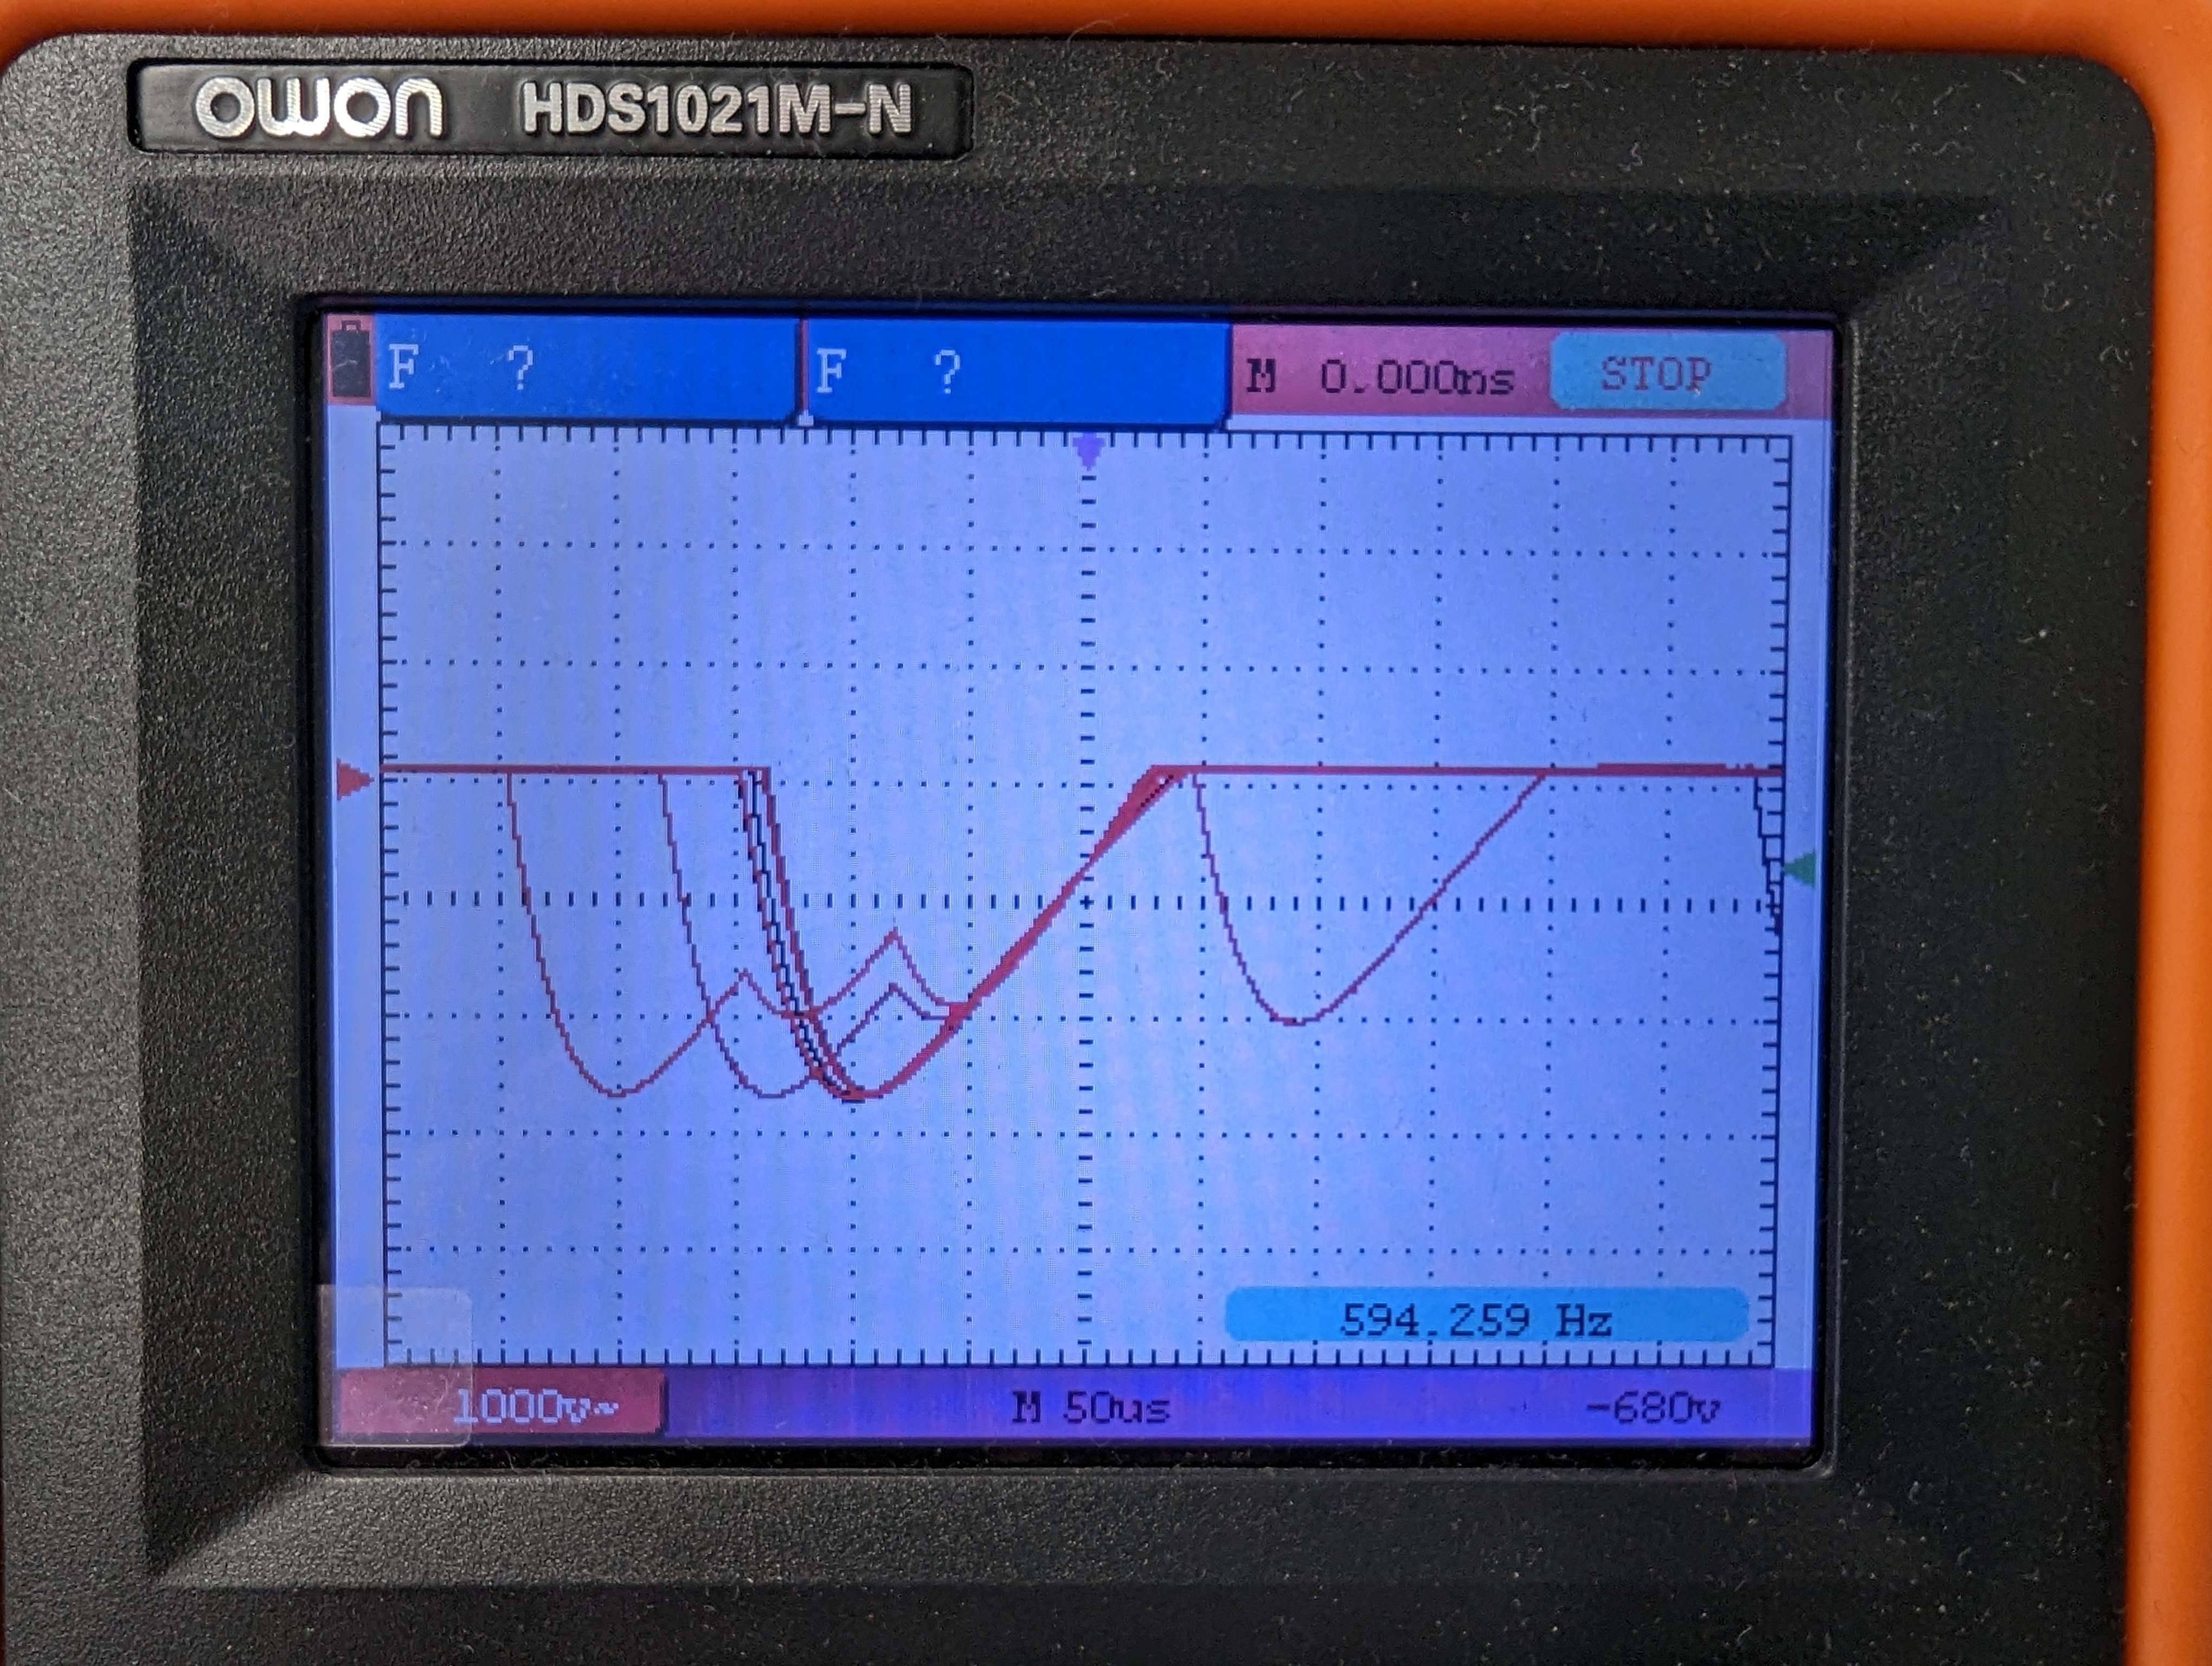
\includegraphics[width=\textwidth]{content/oszilloskop.jpg}
  \caption{Bild des Oszilloskops zur Abschätzung der Totzeit.}
  \label{fig:totzeit}
\end{figure}
\section{Diskussion}
\label{sec:Diskussion}
Die Abweichungen der berechneten Größen von der Theorie werden nach 
\begin{equation}\label{1}
    \Delta = |\frac{exp - theo}{theo} \cdot 100|
\end{equation}
berechnet.
\subsection{Die Wellenlänge des Lasers}
Der verwendete Laser emittiert Licht mit einer Wellenlänge von $\lambda_{real} = \SI{680}{nm}$. Dadurch ergeben sich die in \autoref{tab:abw1} dargestellten
prozentualen Abweichungen von der Angabe des Lasers.
\begin{table}[H]
    \centering
    \caption{Berechnete Wellenlänge $\lambda$ und reale Angabe $\lambda_{real}$}
    \begin{tabular}{c c}
        \toprule
        $\lambda \,[\unit{nm}]$ & $\Delta\,[\unit{\%}]$\\
        \midrule
        $\SI{717(14)}{}$ & 5.4\\
        $\SI{808(16)}{}$ & 18.8\\
        \bottomrule
    \end{tabular}
    \label{tab:abw1}
\end{table}


\printbibliography{}

\section{Messdaten}\label{Messdaten}

\begin{figure}[H]
    \includegraphics[width=15cm,height=20cm]{fotos/messdaten1.jpg}
    \caption{Messdaten 1}
\end{figure}

\begin{figure}[H]
    \includegraphics[width=15cm,height=20cm]{fotos/messdaten2.jpg}
    \caption{Messdaten 2}
\end{figure}

\begin{figure}[H]
    \includegraphics[width=15cm,height=20cm]{fotos/messdaten3.jpg}
    \caption{Messdaten 3}
\end{figure}

\end{document}
